\chapter{Angle control between satellites}
In this chapter, the focus will be on modelling and the control of the angle between two satellites using the drag force as the control input of the system. In this section the satellite is able to change its orientation instantaneously, therefore the drag force can be modified instantaneously. The Earth and the satellite are assumed to be a point mass to simplify the system. 
\section{Modelling}
The satellite is mainly subjected to three forces: the gravity, the drag force and the solar radiation. Thus, the second law of Newton gives:
\begin{flalign}
 \sum \vec {F} = m_{sat} \ \vec a = \vec{F_g} + \vec{F_D} + \vec{F_{rad}}
	\label{eq:ecc}
\end{flalign}
with the gravity modeled by:
\begin{flalign}
{F_g} = -G\frac{m_{earth} m_{sat}}{||\vec{p}||^3} \vec{p}
	\label{eq:eccc}
\end{flalign}
where $\vec{p}$ is the vector position of the satellite from the Earth centre to the mass centre of the satellite in the inertial frame and the expression for ${F_D}$ and ${F_{rad}}$ are explained in the next section.
\section{Disturbance Models}
\subsection{Aerodynamic Drag Force}
The satellite is subjected to an aerodynamic drag force due to the atmosphere. The collisions with the air cause a force in the opposite direction of the velocity of the satellite. The force was modelled by Lord Rayleigh.\cite{FSA}
\begin{flalign}
\vec{F_D} = -\frac{1}{2} \rho \ C_D \ A_{\perp} ||\vec{v}||  \vec{v}
	\label{eq:ec1c}
\end{flalign}
where $\rho$ is the density of the air, $C_D$ is the drag coefficient, $A_{\perp}$ is the area that is perpendicular of the velocity of the satellite $\vec{v}$. 

The drag coefficient $C_D$ and the perpendicular area $A_{\perp}$ depend on the orientation of the satellite. Therefore, this force can be used as an input for the control of the position and the velocity of the satellite.

The density of the air depends on the altitude of the satellite and the air temperature, but it is considered to be constant in this case for simplifying the model. $\rho$ is chosen to be equal to $1.454 \cdot 10^{-13} Kg/{m^3}$ based on the  empirical model of the Committee on Space Research (COSPAR) International Reference Atmosphere \cite{FSA}.

The drag coefficient is dependent on the orientation and the maximum value of $C_D$ is equal to 1.05 for a non tilted cubed as shown on the \figref{fig:drag} and equal to 0.80 for an angled cubed \cite{wik}. The drag coefficient is assumed to be constant and equal to 1 in order to simplify the equation. 
\begin{table}[H]
	\begin{minipage}[b]{0.49\linewidth}
		\centering
		\begin{figure}[H]
			\centering
			\includegraphics[width=0.8\linewidth]{figures/drag_coef}
			\caption{description needed}
			\label{fig:drag}
		\end{figure}
	\end{minipage}\hfill
	\begin{minipage}[b]{0.49\linewidth}
		\centering
		\begin{figure}[H]
			\centering
			\includegraphics[width=1\linewidth]{figures/a_prep}
			\caption{description needed}
			\label{fig:cub}
		\end{figure}
	\end{minipage}
\end{table}
Therefore, the control parameter is the perpendicular area $A_{\perp}$. The maximum and minimum value of $A_{\perp}$ is represented in \figref{fig:cub}. Thus, the minimum value is the surface of a square of 10cm of dimension ($A_{\perp} = 100cm^2$) and the maximum value is the surface of an hexagon of 10cm of dimension ($A_{\perp} = \frac{3\sqrt{3}}{2} 100cm^2$).
Thus, the drag force can be expressed as the following. 
\begin{flalign}
\vec{F_D} = -u ||\vec{v}|| \vec{v}
\label{eq:teor}
\end{flalign}
where $u$ is the control input and it can take value between $7.27 \cdot 10^{-16}$ and $1.888 \cdot 10^{-15}$
\subsection{Solar radiation}
Solar radiation is emitted constantly by the Sun, which illuminates the surface of the CubeSat. The surface of the satellite will absorb or reflect the solar radiation, nevertheless, these two situations will alter the CubeSat and produce a radiation force. \cite{SADC}

The solar flux can be computed as follows:
\begin{flalign}
	P = \dfrac{F_s}{c}
	\label{eq:flux}
\end{flalign}
where $F_s$ is the mean solar energy and it is equal with 1358 $W/m^2$ and $c$ is the speed of light

The solar radiation $F_{rad}$ can be expressed as:
\begin{flalign}
\vec {F_{rad}} = C_{a} P A \ \frac{\vec {r_{sun,sat}}}{||\vec {r_{sun,sat}}||}
\label{eq:Pres}
\end{flalign}
where $C_{a}$ is the surface’s reflectance: 0 for a perfect absorber, 2 for a perfect reflector, $P$ is the solar flux, $A$ is the radiated area, $r_{sun,sat}$ is the vector from the sun to the satellite and the norm of $||r_{sun,sat}||$ is equal to 1

\subsection{$J_2$ gravity perturbation}
The force which the Earth is exerting upon a object outside its sphere is a conservative force and its potential energy can be written as follows:
\begin{flalign}
	U(r) = -\frac{\mu}{r}
	\label{eq:Pr}
\end{flalign}
Because the Earth is not a perfect sphere and also its mass distribution is not homogeneous, \eqref{eq:Pr} is rewritten by adding the spherical harmonic expansion to correct the gravitational potential for the Earth:
\begin{flalign}
		U(r) = -\frac{\mu}{r}+ B(r, \phi , \lambda)
	\label{eq:Pr1}
\end{flalign}
where $B(r, \phi, \lambda)$ is the spherical harmonic expansion used to correct the gravitational potential for the Earth's nonsymmetric mass distribution seen in \figref{fig:j2}
\begin{figure}[H]
	\centering
	\includegraphics[width=0.6\linewidth]{figures/j2}
	\caption{Coordinates for deriving the external gravitational potential of the Earth }
	\label{fig:j2}
\end{figure} 
In order to solve the problem regarding the oblatness, the gravitational potential of the Earth is extended into series of spherical harmonics: [ref]
\begin{flalign}
	 B(r, \phi , \lambda) = \frac{\mu}{r} \left\{ \sum_{n=2}^{\infty} \left [ \left (\frac{R_e}{r} \right)^{n} J_n P_n sin(\phi)| +\sum_{m=1}^{n} \left (\frac{R_e}{r}\right)^{n} (C_{nm} cos(m\lambda) + S_{nm} sin(m\lambda)) P_{nm} sin(\phi)  \right] \right\}
	\label{eq:phi2}
\end{flalign}
where $r, \phi , \lambda$ are spherical coordinates and the parameteres from the function are defined as follows: $r$ is the geocentric distance of point $P$, $\phi$ is the geocentric latitude, $\lambda$ is the geographical longitude, $R_e$ is the mean equatorial radius of the Earth, $cos(m\lambda)$ and $sin(m\lambda)$ are harmonics in $\lambda$, $J_{nm}$ are the zonal harmonic coefficients, $J_n$ zonal harmonic coefficients of order 0, $P_{nm} $ associated Legendre polynomial of degree $n$ and order $m$, $P_n$ is Legendre polynomial degree $n$ and order 0, $C_{nm}$ is tesseral harmonic coefficients for $n \neq m$, $S_{nm}$ is sectoral harmonic coefficients for $n =m$

The expression for gravitational potential of the Earth can be approximate as:
\begin{flalign}
   U \approx -\frac{\mu}{r} \left[1 - \sum_{n=2}^{\infty} \left(\frac{R_e}{r}\right)^{n} J_n P_n sin(\phi)  \right ] = \frac{\mu}{r} [U_0 + U_{J_2} + U_{J_3} + ...]
	\label{eq:Pr341}
\end{flalign}
where $U_0$ = -1 and $U_{J_2}$ = $\left(\frac{R_e}{r}\right)^{2} J_2 \frac{1}{2} (3 sin^2 \phi -1) $

The gravitational forces acting on the satellite are obtained from the relation:
\begin{flalign}
	F = -m \nabla U
	\label{eq:Pr3431}
\end{flalign}
and is obtaining the following:
\begin{flalign}
	F_x = -\frac{\partial U}{\partial x} = \mu \left[ -\frac{x}{r^3} + A_{J_2} \left(15 \frac{xz^2}{r^7} - 3\frac{x}{r^5}   \right ) \right ]       \\
		F_y = -\frac{\partial U}{\partial y} = \mu \left[ -\frac{y}{r^3} + A_{J_2} \left(15 \frac{yz^2}{r^7} - 3\frac{y}{r^5}   \right ) \right ]       \\
			F_z = - \frac{\partial U}{\partial z} =  \mu \left[ -\frac{z}{r^3} + A_{J_2} \left(15 \frac{z^3}{r^7} - 3\frac{z}{r^5}   \right )  \right]       
	\label{eq:Pr34331}
\end{flalign}
where $A_{J_2}  = \frac{1}{2} J_2 R_e^2$ and and$R_e$ is the mean radius ofthe earth at the equator
	
\section{State Space Representation}
The state of the system is the vector position and the vector velocity in the inertial frame:
\begin{flalign}
{x} = \left[ \begin{array}{c} \vec{p} \\ \vec{v} \end{array} \right]
	\label{eq:Pr3341}
\end{flalign}
The equation is given by:
\begin{flalign}
\dot{x} &= \left[ \begin{array}{c} \dot{p} \\ \dot{v} \end{array} \right] = \left[ \begin{array}{c} {v} \\ {a} \end{array} \right] \\
 &= \left[ \begin{array}{c} \vec{v} \\ \frac{1}{m_{sat}}(-G\frac{m_{earth}  m_{sat}}{||{p}||^3} {p} - u ||\vec{v}|| \vec{v}) + {\delta(x,t)} \end{array} \right] \\
 &= {f(x)} + u \cdot {g(x)} + {\delta(x,t)}
\end{flalign}
with 
\[
{f(x)} = \left[ \begin{array}{c} {v} \\ -G\cdot m_{earth} \frac{p}{||{p}||^3} \end{array} \right], \ {g(x)} = \left[ \begin{array}{c} {0} \\ - \frac{1}{m_{sat}}||{v}||{v} \end{array} \right]
\]
and ${\delta(x,t)}$ reprensent the influence all the disturbances.
\section{Relative dynamics} 
%ref:jesper randevouz article
In order to analyse the distance between two satellites, the relative dynamics are analyzed. Furthermore, to simplify the system, satellites will be assumed to stay on the same plane. This assumption has also to be made due to the limitation of the direction of the input control (the drag force). \\
To compute the equations of the motion of one satellite compared to another, a new frame is used. The frame is illustrated in the \figref{fig:rel_dyn}, where the origin is the first satellite and the axis ${\hat{x}}$ is defined by ${\hat{x}} = \frac{\vec R}{|| \vec R ||}$, where ${R}$ is the vector from the centre of the Earth to the first satellite. The axis ${\hat{y}}$ is perpendicular to ${\hat{x}}$ and in the plane of motion of the satellites and ${\hat{z}}$ is defined by the right-hand law (${\hat{z}} = {\hat{x}} \times {\hat{y}}$). 
\begin{figure}[H]
	\centering
	\includegraphics[width=0.6\linewidth]{figures/relativeDynamics}
	\caption{Frame for the relative dynamics}
	\label{fig:rel_dyn}
\end{figure} 
Therefore, the vector position from the Earth to the fisrt satellite and the second satellite can be expressed in this frame:
\begin{flalign}
\vec{p_1} &= R \  {\hat{x}} \\
\vec{p_2} &= R \  \vec{\hat{x}} + x \ \vec {\hat{x}} + y \  \vec{\hat{y}} 
\end{flalign}
The equations of relative motions are derived in \appref{chap:B}.
%
\subsubsection{Relative state space representation}
Since the equations of relative motion  that have been derived in \appref{chap:B} are not linear, a linearization is made around the operating points, $x^{*}$ and $y^{*}$, by introducing the states with a new variable as $s = [x \ \dot{x} \ y \ \dot{y}]^\mathsf{T}$, furthermore the derivation is made in \appref{chap:C}.  

In order to derive the linear state-space model the assumptions that the radius is constant and that the angular velocity, $w = \sqrt{\frac{\mu}{R^3}}$ is constant, lead to the assumption that $\dot{R} = 0$ and $\dot{w} = 0$. Furthermore, using the approximation $\dot{x}$, $y << y^{*}$ and $x, x^{*}$, $\frac{\dot{y}}{w} << R$, the \eqref{eq:statespaceassumption} has been derived. Finally assuming that $y^{*} << R$ the linear system can be written in state space form as follows: 
 \begin{flalign*}
 	{\dot{s}(t)} ={A x(t) + Bu(t)} 
 \end{flalign*}  
\begin{flalign*}
	{A}
	= 
	\begin{bmatrix}
		0& 1& 0 & 0 \\
		0& 0&0&2w  \\ 
		0&0&0&1 \\
		0&-2w & 0 &0
	\end{bmatrix} 
\end{flalign*}
\begin{flalign*}
	{B}
	= 
	\begin{bmatrix}
		0& \\
		0&  \\ 
		0& \\
		-Rw&
	\end{bmatrix} 
\end{flalign*}
With this assumptions and by using a control law $u= u_2 - u_1$ from the \eqref{eq:statespaceassumption} it can be seen that when $u_2 > u_1$ then $u>0$ and in this case $y$ should decrease as seen in \figref{fig:u1}. From \figref{fig:u2} it can be seen that the theoretical and the practical of $y$  are not the similar. This is due to the fact that when a satellite is subject to a drag force, the altitude of the satellite is decreasing and the angular velocity is increasing, which will be shown in the next section.
\begin{table}[H]
	\begin{minipage}[b]{0.49\linewidth}
		\centering
		\begin{figure}[H]
			\centering
			\includegraphics[width=1\linewidth]{figures/theoryapprox.eps}
			\caption{Approximation model}
			\label{fig:u1}
		\end{figure}
	\end{minipage}\hfill
	\begin{minipage}[b]{0.49\linewidth}
		\centering
		\begin{figure}[H]
			\centering
			\includegraphics[width=1\linewidth]{figures/practiceapprox.eps}
			\caption{Real model}
			\label{fig:u2}
		\end{figure}
	\end{minipage}
\end{table}
Therefore, when $u_2 > u_1$, then $w_2 > w_1$ this will lead to an increase in the angle $\theta$ between the satellites, and since $y = R \ sin\theta$, $y$ will have an increasing attitude. The above mentioned issues are shown in \figref{fig:u2}.

In conclusion, the approximation that the time derritve of angular velocity is equal to 0 cannot be made for controlling the distance of the two satellites.
\section{Modelling based on the angular velocity}
As seen in the previous section, the angular velocity cannot be assumed constant. Therefore an equation is needed to estimate it as a function of the drag force. In \appref{chap:C}, the time derivative of the angular velocity can be approximated as a linear function of the drag force. 
\begin{flalign}
	{\Delta \dot\omega} = C u
	\label{eq:u3}
\end{flalign}
with $C = \frac{3 \omega_0^2 R_0}{m}$. In order to check this equation and the coefficient, a simulation is performed using a constant drag force coefficient ($u = \frac{u_{min} + u_{max}}{2}$). The angular velocity as a function of time with constant drag force is shown in \figref{fig:testCoef}. \\
\begin{figure}[H]
	\centering
	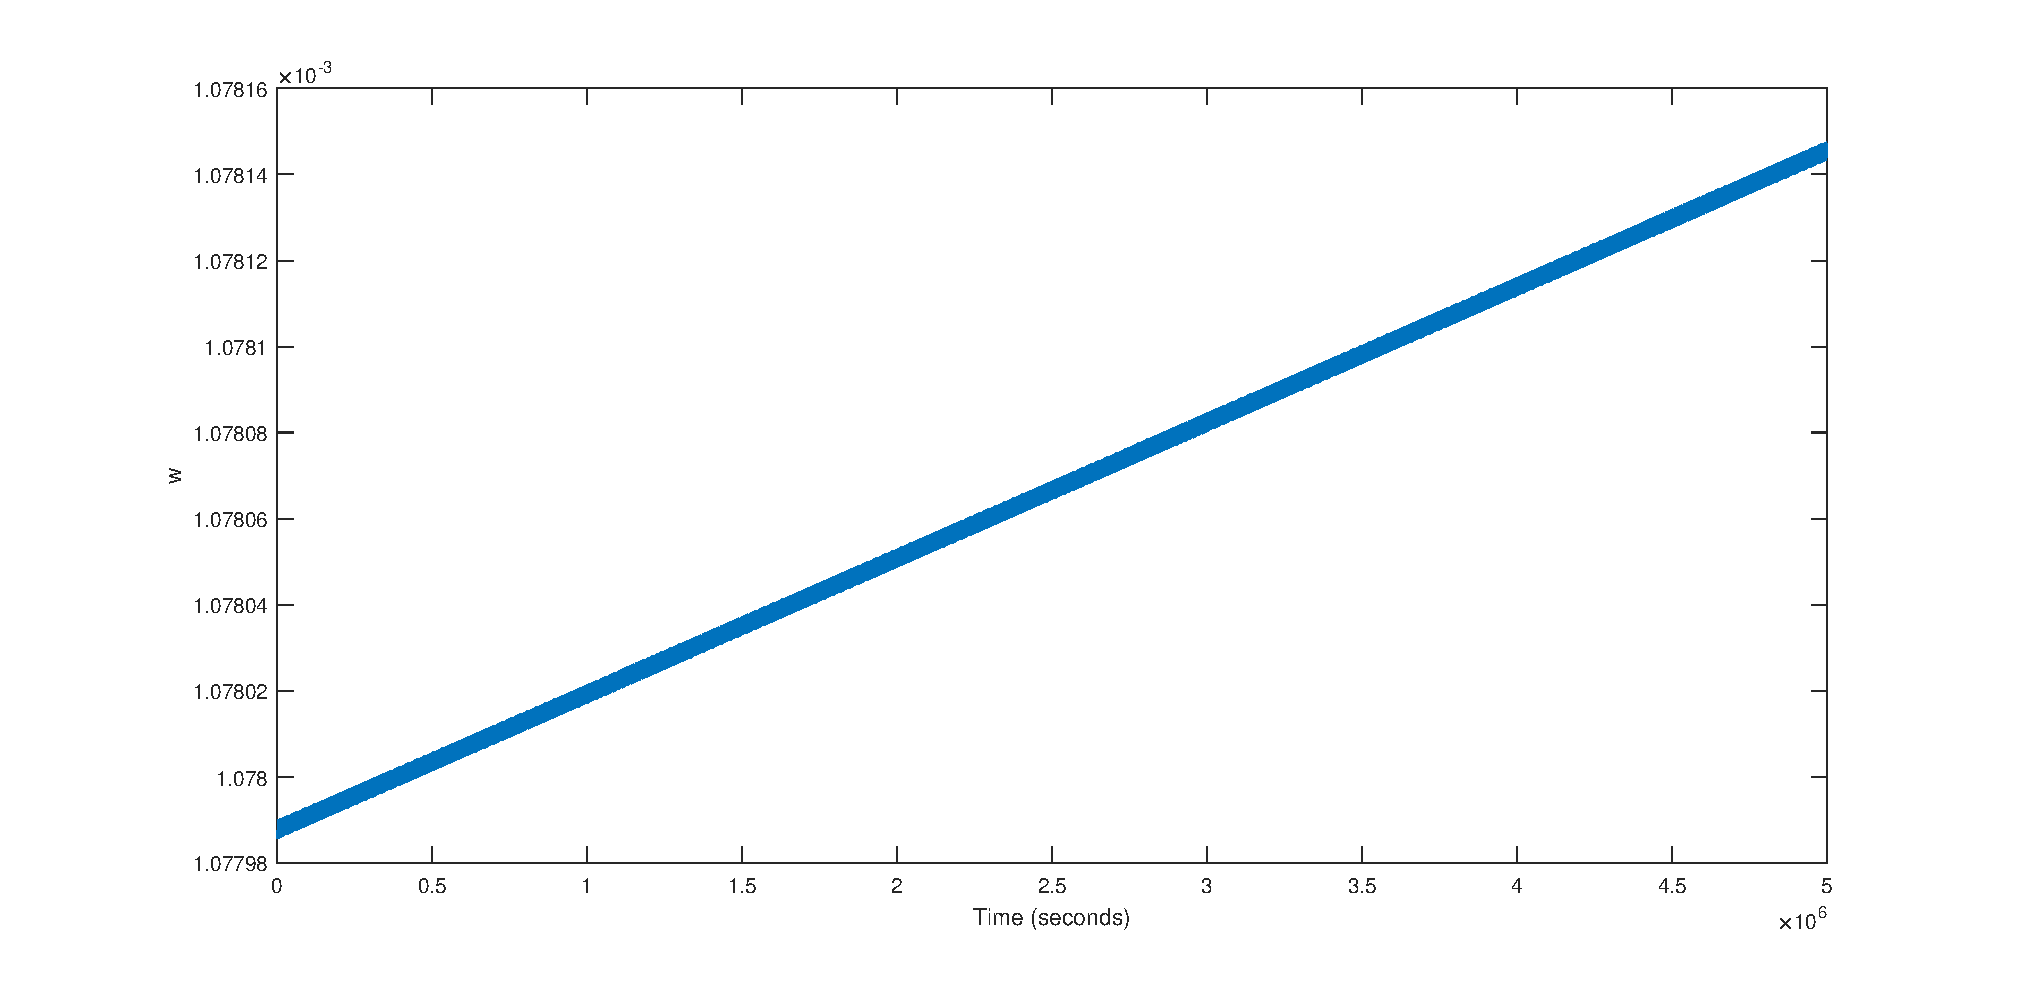
\includegraphics[width=0.9\linewidth]
	{figures/test_coef.eps}
	\caption{Angular velocity as function of time}
	\label{fig:testCoef}
\end{figure} 
The coefficient found in the simulation is almost the same than in the theory and oscillations can be observed with a frequency equals to $f \approx \frac{2\pi}{\omega_0}$. This is due to the fact that the orbit is not exactly a circle but an ellipse. Thus, the angular velocity changes slightly during a turn around the Earth. In order to limit the influence of these variations on the controller, a second order low pass filter is added to reduce the amplitude of these oscillations. A state space representation can be derived with states $\theta$ and $\dot \theta$, where $\theta$ is the angle between two satellites. The time derritve of $\dot \theta$ is equal with $\dot \omega_2 - \dot \omega_1$ and using \eqref{eq:u3}, $\ddot \theta = C   u_2 - C u_1 = C u$.
\begin{flalign}
	{s}
	= 
	\begin{bmatrix}
		\theta  \\
		\dot{\theta}
	\end{bmatrix} 
\end{flalign}
\begin{flalign}
	&{\dot{s}(t)} ={A s(t) + Bu(t)}  	\label{eq:lt}
\end{flalign}  
where
\begin{flalign}
	{A}
	= 
	\begin{bmatrix}
		0& 1& \\
		0& 0&
	\end{bmatrix} 
\end{flalign}
\begin{flalign}
	{B}
	= 
	\begin{bmatrix}
		0& \\
		\frac{3 \omega_0^2 R_0}{m}
	\end{bmatrix} 
\end{flalign}
\section{Distance control design}
A controller is designed to control the angle between two satellites. Due to the fact that the state representation is linear, Linear Quadratic Regulator(LQR) is chosen as control method with the following cost function:
\begin{flalign}
\mathcal{I} =  \int (\vec{x}^\mathsf{T} \ \underline{Q} \ \vec{x} + \vec{u}^\mathsf{T} \ \underline{R}  \ \vec{u}) dx
\end{flalign}
where $Q$ and $R$ are weighting matrices chosen as: \label{ref}
\begin{flalign}
	{Q}
	= 
	\begin{bmatrix}
		(\frac{pi}{3})^{-2}& 0& \\
		0& 0&
	\end{bmatrix} 
\end{flalign}
\begin{flalign}
	{R}
	= 
	\begin{bmatrix}
		u_{max}^{-2}
	\end{bmatrix} 
\end{flalign}
 The vector of gain K is obtained using the command \textit{lqr(A,B,C,D,[])} in Matlab. The control input signal can be computed ($u = u_2 - u_1$) and therefore if u is bigger than zero, $u_1$ will be equal to $u_{min}$ and $u_2$ will be equal to $u + u_{min}$. If u is smaller than zero, it will be the opposite.
 The control law used for designing the controller is: $u = -K(1) \ \theta \ -K(2) \ \dot \theta $. \label{eq:ctr}
\subsection{Frequency Analysis}
The loop transfer function can be computed $L(s) = P(s) \ C(s) \ LPF(s)$ where $P(s$ is the transfer function of the state representation system, $C(s) = K_1 + K_2 s$ is the transfer function of the controller and $LPF(s)$ is the transfer function of the second order low pass filter.
The bode diagram of L(s) is represented in the \figref{fig:Bode_L}. \\
\begin{figure}[H]
	\centering
	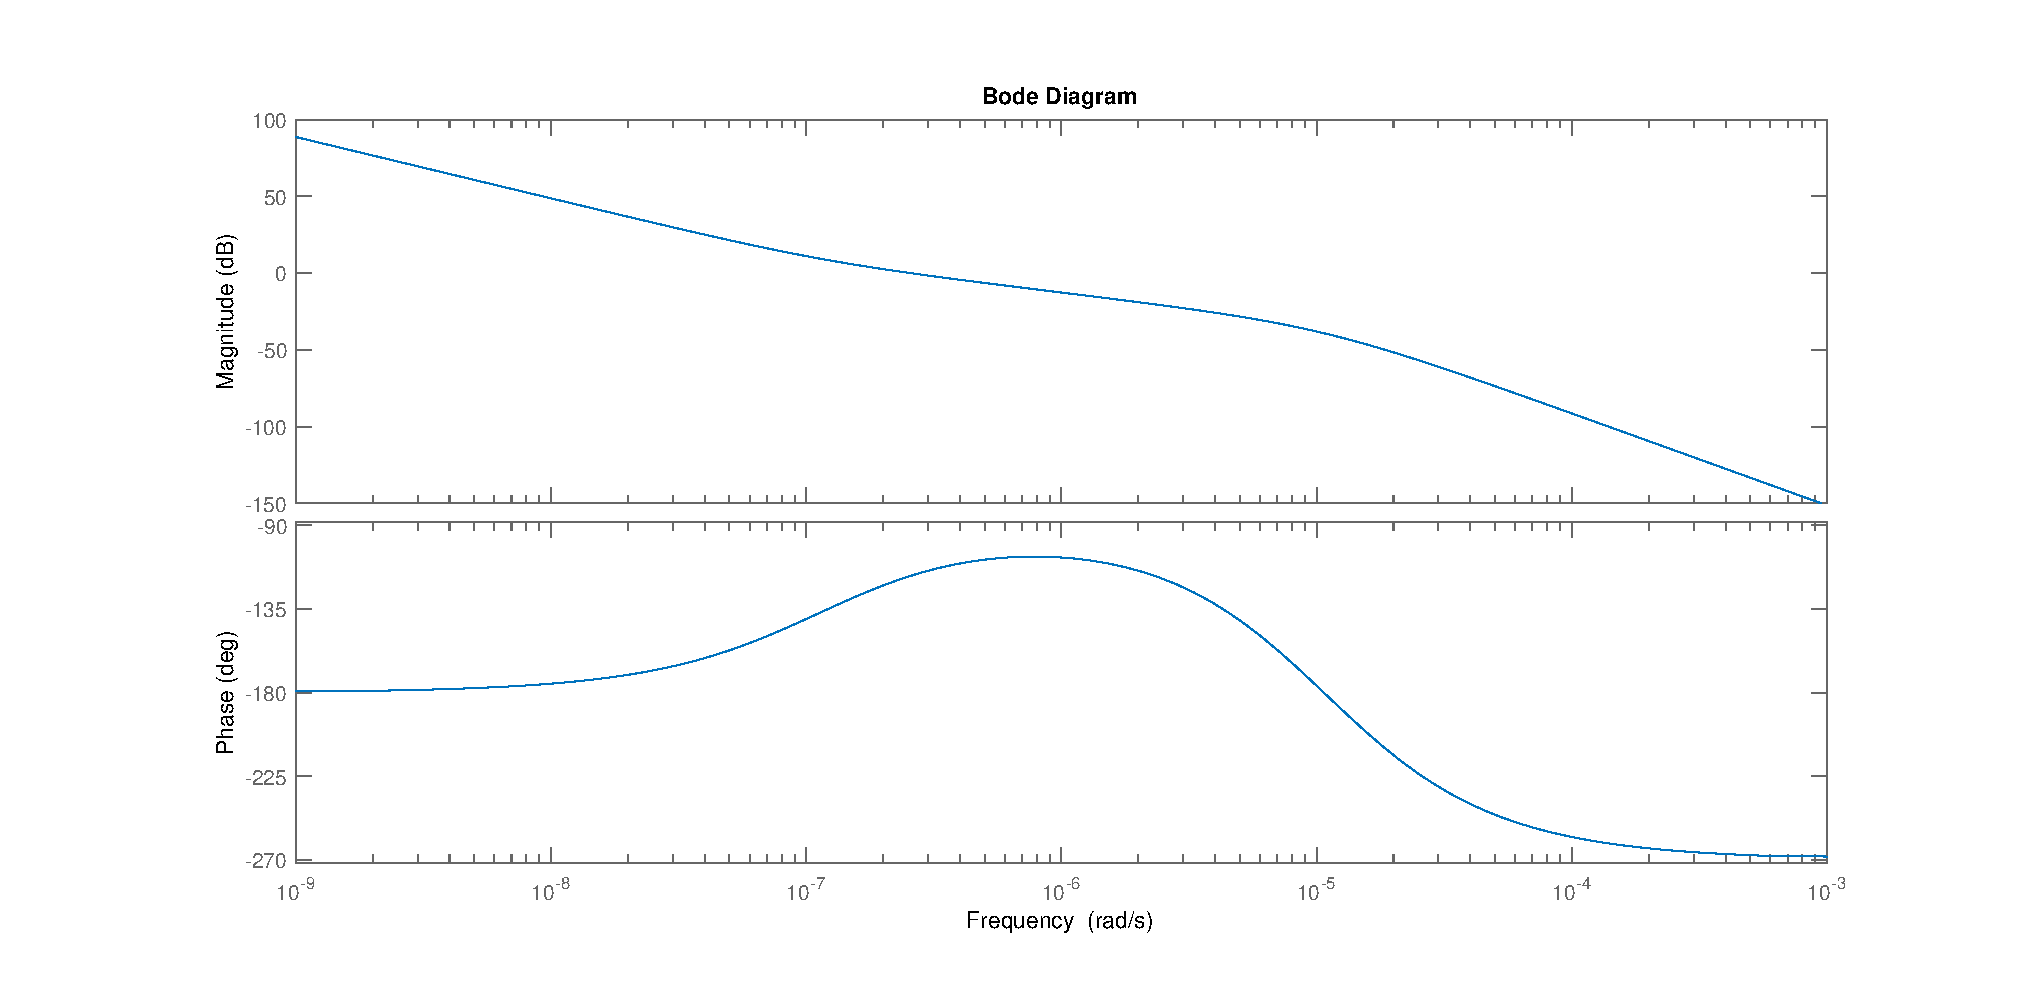
\includegraphics[width=0.9\linewidth]
	{figures/Bode_L.eps}
	\caption{Bode diagram of the loop transfer function}
	\label{fig:Bode_L}
\end{figure}
In the modelling, the control input signal (drag force coefficient) was assumed to be able to change instantaneously but in the real system, variations of the orientation of the satellite take times. Therefore, the phase margin must be big enough to allow a delay in the controller. In the bode diagram, the phase margin can be estimated equal to 60$^{\circ}$  which is enough to accept a large delay due to the small crossover frequency. \\
\subsection{Satellite Formation Control} 
\subsubsection{Global algorithm}
Since the formation consists of more than two satellites a second controller is designed to control n satellites around the Earth. The gain vector K computed above can be used to calculate the difference drag force between two neighbours satellites (called $u_a = u_2 - u_1$, $u_b = u_3 - u_2$, ...). Thus, a system of $n-1$ equations with n unknown variables is obtained. the last equation is chosen to set the minimum value of $u_1$, $u_2$,... equals to $u_{min}$. We have now a system of $n$ equations with $n$ unknown variables that can be solved to determine the drag force coefficient $u_i$ for each satellite.
\subsubsection{Distributed algorithm}
In this case, $u_1$ is chosen to be equal with $u_{medium}$, therefore $u_2$ is computed using the control law found in \eqref{eq:ctr}, which is a function of the angle between the first satellite and the second one. The drag force of satellite $i$ can be determined by knowing the angle between the satellite $i$ and $i-1$, the time derivative of this angle and the drag force of the satellite $i-1$.
\subsection{Stability Analysis}
In order to analyze the stability of the distributed formation controller, the global system is written in state space form as in  \eqref{eq:lt}. The states are defined as 
\begin{flalign*}
	s = [\theta_n \ \dot{\theta_n}]^\mathsf{T}
	\label{stateformation}
\end{flalign*}
where $\theta_n = [\theta_{12} \ \theta_{23} \ \theta_{34} \ \theta_{45} \ \theta_{56} \ \theta_{67} \ \theta_{78}]^\mathsf{T}$ are the angles between neighbour satellites and $\dot{\theta_n} $ is the time derivative of these angles. The system matrix will be a 14x14 matrix and for $i<8$ satellites, $\dot{s}_{i} = s_{i+7}$. Therefore the $A$ and $B$ matrix can be written as:

	$
	A = \left(\begin{array}{c@{}c@{}c}
    0_{(7\times7)} & | & I_{(7\times7)}\\
	\hline
	  & 0
	\end{array}\right),
	B = \left(\begin{array}{c@{}c@{}c}
	& 0_{(7\times7)} \\
	\hline
	& C \ I_{(7\times7)}
	\end{array}\right)
	$
with the constant $C = \frac{3 \omega_0^2 R_0}{m} $ and $u = [u_2-u_1;u_3-u_2;...;u_8-u_7]$.

The controller gain that has been found in section \ref{ref}, $K = [K_{1} \ K_{2}]$, now can be written as $K_{s} = [K_{1}I_{(7\times7)},  \ K_{2}I_{(7\times7)}]$ and  by using a control law $u = -Ks$ a stability analysis can be made using a Lyapunov candidate function $V = s^{T}s$ where $V>0$, $\forall s\neq0 $. Inserting $K_{s}$, the state space equation becomes:
\begin{flalign}
	&{\dot{s}} ={(A  + BK_{s})s}
	\label{eq:statespacecomplex2}
\end{flalign}  
%
From Lyapunov stability criterion, it has to be shown that $\dot{V} <0$,$\forall s\neq0 $. The derivative of the candidate function can be written as 
%
\begin{flalign}
	&{\dot{V}} ={\dot{s}^\mathsf{T}s+s^\mathsf{T}\dot{s}}
	\label{eq:statespacecomplex3}
\end{flalign}
%
and this is equal to 
%
\begin{flalign}
	&{\dot{V}} ={s^\mathsf{T}(A-BK)^\mathsf{T}s + s^\mathsf{T}(A-BK)s}
	\label{eq:statespacecomplex4}
\end{flalign}
so the only thing that has to be shown in order the system to be stable is to show that the all the eigenvalues of $A-BK<0$. The eigenvalues $A-BK$ were computed using Matlab and the result was that the all eigenvalues have negative real part.
\section{Simulation and results}
 First, the simulation results of the control scheme between two satellites are shown. After the results of two satellites, the results for the whole satellite formation are shown with global and distributed algorithm. The reference angle is chosen to be $60^{o}$ for two satellites case and $45^{o}$ for the whole formation. The inputs to the controller are $\Delta\theta$ and $\dot{\theta}$, where $\Delta\theta = \theta - \theta{ref}$ and $\dot{\theta} = w_2 - w_1$. In order to smooth the high frequency  oscillations from $\theta$, $w_1$ and $w_2$ to the controller a low pass filter is used. The control design is similar to PD controller. In \figref{fig:distancecontrol} is shown the response of the controller and in \figref{fig:distancecontrol2} the angle between two satellites. The settling time is $2\times10^7$ which is equivalent to 230 days which is satisfactory, and also no saturation in the drag force appears.
\begin{table}[H]
	\begin{minipage}[b]{0.49\linewidth}
		\centering
		\begin{figure}[H]
			\centering
			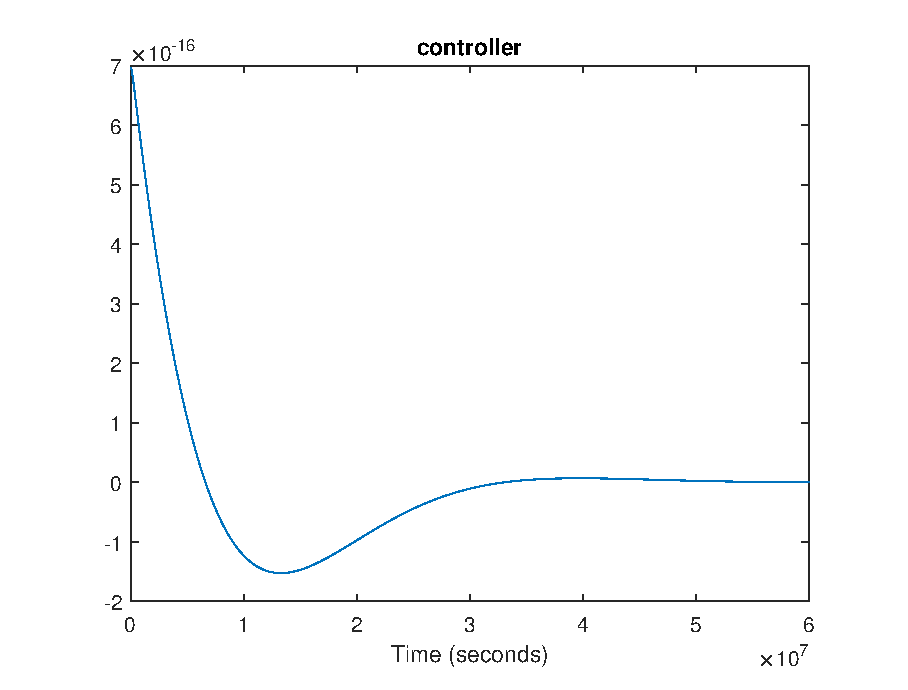
\includegraphics[width=1\linewidth]{figures/distance_control_twosat.eps}
			\caption{ Distance control of two satellites}
			\label{fig:distancecontrol}
		\end{figure}
	\end{minipage}\hfill
	\begin{minipage}[b]{0.49\linewidth}
		\centering
		\begin{figure}[H]
			\centering
			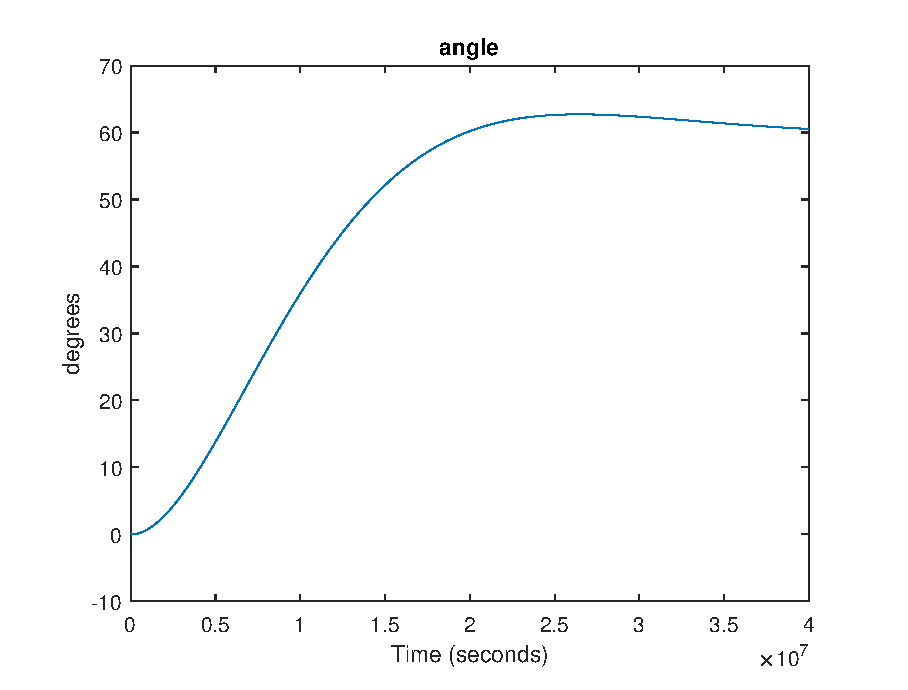
\includegraphics[width=1\linewidth]{figures/newangle.eps}
			\caption{Angle between two satellites}
			\label{fig:distancecontrol2}
		\end{figure}
	\end{minipage}
\end{table}

The \figref{fig:distancecontrol3} and \figref{fig:distancecontrol4} show the input signal to the satellite 1 and satellite 2 respectively.
\begin{table}[H]
	\begin{minipage}[b]{0.49\linewidth}
		\centering
		\begin{figure}[H]
			\centering
			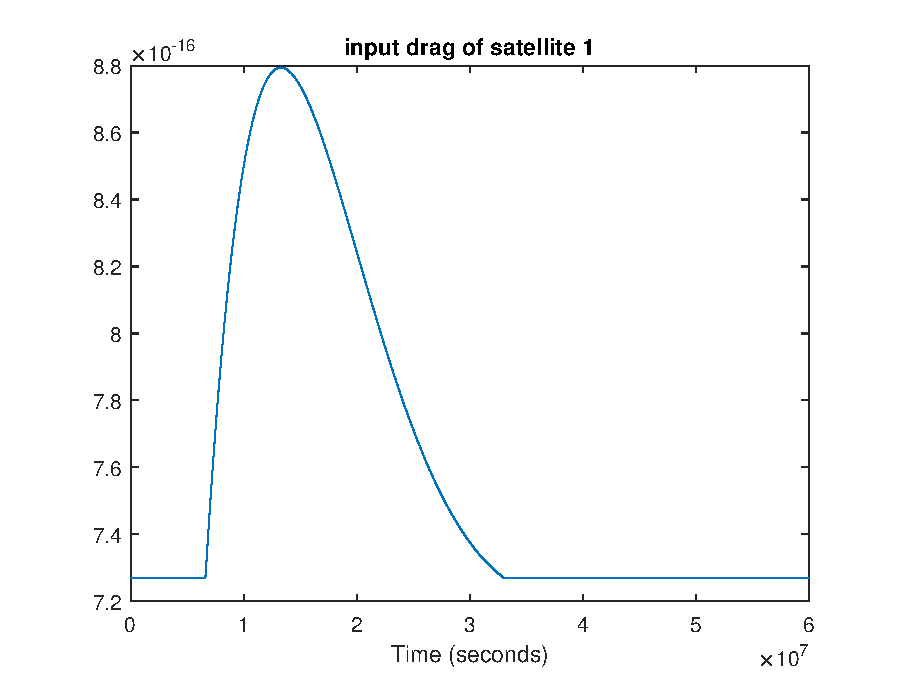
\includegraphics[width=1\linewidth]{figures/input_drag_sat1.eps}
			\caption{ The applied input of satellite 1 }
			\label{fig:distancecontrol3}
		\end{figure}
	\end{minipage}\hfill
	\begin{minipage}[b]{0.49\linewidth}
		\centering
		\begin{figure}[H]
			\centering
			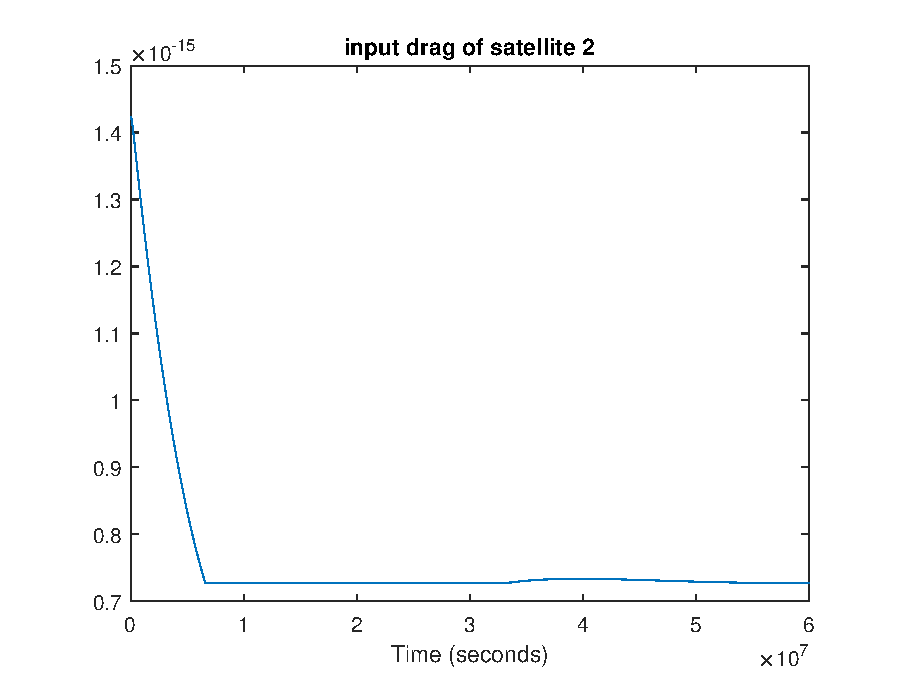
\includegraphics[width=1\linewidth]{figures/input_drag_sat2.eps}
			\caption{The applied input of satellite 2}
			\label{fig:distancecontrol4}
		\end{figure}
	\end{minipage}
\end{table}
\subsection{Global algorithm results}
The behaviour of the satellite formation using global algorithm was tested according to a hypothesis that the satellite formation starts at the same place. From \figref{fig:forr} it can be seen that in the beginning, some saturation appears, but finally, all the satellites converged to the desired angle of 45$^{\circ}$ .
\begin{figure}[H]
	\centering
	\includegraphics[width=1\linewidth]{figures/form_sat}
	\caption{Eight satellites in flying formation on orbit}
	\label{fig:forr}
\end{figure}
\subsection{Distributed algorithm results}
In the case of a distributed algorithm, the behaviour of the satellite formation is shown in \figref{fig:da1}, where it can be seen that the overshoot is big, therefore in order to reduce the overshoot, the derivative gain is increased by a factor of 1.25, which will correct the overshoot as seen in  \figref{fig:da1}.
\begin{table}[H]
	\begin{minipage}[b]{0.49\linewidth}
		\centering
		\begin{figure}[H]
			\centering
			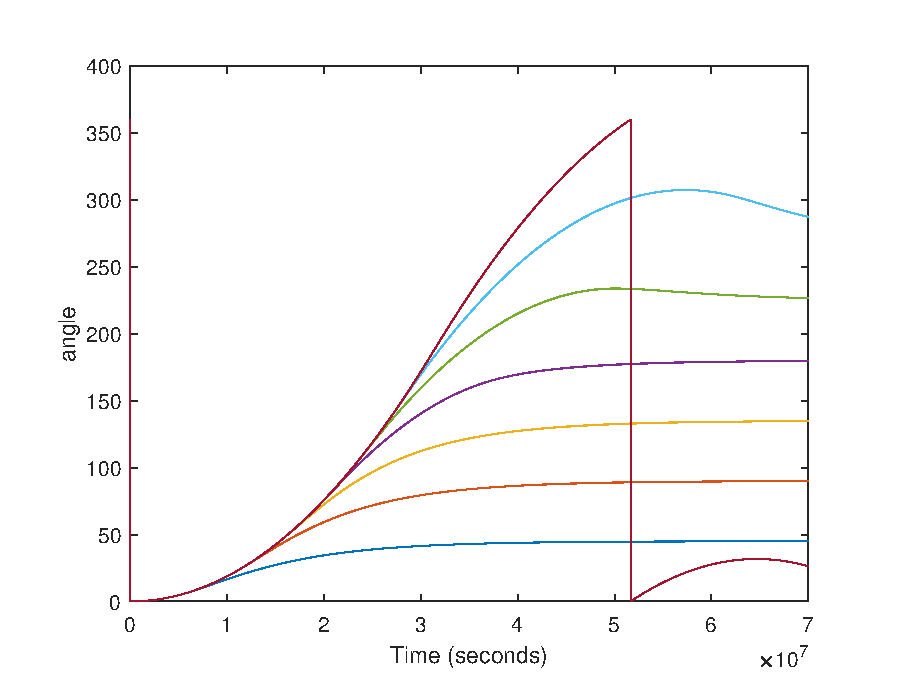
\includegraphics[width=1.1\linewidth]{figures/da1}
			\caption{ asd }
			\label{fig:da1}
		\end{figure}
	\end{minipage}\hfill
	\begin{minipage}[b]{0.49\linewidth}
		\centering
		\begin{figure}[H]
			\centering
			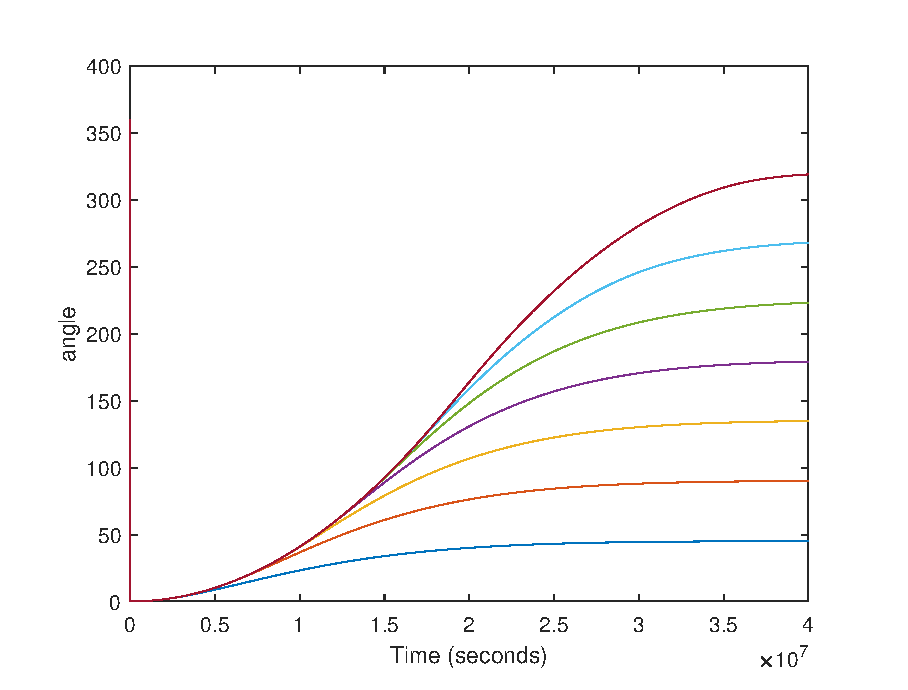
\includegraphics[width=1.1\linewidth]{figures/da2}
			\caption{asd }
			\label{fig:da2}
		\end{figure}
	\end{minipage}
\end{table}
The drawback of distributed algorithm is that the angle between satellites will converge slower compared with the global algorithm, moreover, all the satellites are converging to $u_{min}$, while in the case of distributed algorithm are converging to $u_{medium}$